\documentclass[a4paper,12pt,twoside]{book}
\usepackage[utf8]{inputenc}

\usepackage{graphicx}
\usepackage[colorlinks=true, allcolors=blue]{hyperref}
\usepackage[a4paper,top=2cm,bottom=2cm,left=2.5cm,right=2.5cm]{geometry}
\usepackage{amsthm,amssymb,amsmath,amsfonts}
\usepackage{booktabs,ragged2e,ptext}
\usepackage[dvipsnames]{xcolor}
\usepackage{stmaryrd}
\usepackage{subcaption}
\usepackage{url}
%%%%%%%%%%%%%%%%%%%%%%%%%%%%%%%%%%%%%%%%%%%%%%
\usepackage{xepersian}
\settextfont{XB Niloofar}
\setlatintextfont{Times New Roman}
\settextdigitfont[Scale=0.9]{Yas.ttf}
\defpersianfont\mitra{B Mitra.ttf}
\defpersianfont\lotus{Digi Lotos Bold.ttf}
\defpersianfont\estedad{Estedad-Regular.ttf}
%%%%%%%%%%%%%%%%%%%%%%%%%%%%%%%%%%%%%%%%%%%%%%
%% HEADERS AND FOOTERS:
\usepackage{fancyhdr} % Required for customizing headers and footers
\pagestyle{fancy} % Enable the custom headers and footers
\renewcommand{\headrulewidth}{0.5pt} % Top horizontal rule thickness
\fancyhf{} % Clear default headers and footers
\fancyhead[LE, RO]{\sffamily\thepage} % Header for left even pages and right odd pages
\fancyhead[LO]{\rightmark} % Header for left odd pages
\fancyhead[RE]{\leftmark} % Header for right even pages
\fancypagestyle{plain}{ % Style for when a plain pagestyle is specified
	\fancyhead{} % Clear headers
	\renewcommand{\headrulewidth}{0pt} % Remove header rule
}
\usepackage{emptypage} % This package removes headers and footers on empty pages between chapters
%%%%%%%%%%%%%%%%%%%%%%%%%%%%%%%%%%%%%%%%%%%%%%
\linespread{1.2}

\begin{document}

\author{علی عاشوری}
\title{سفر ریاضی}
%\date{January 2013}

\begin{titlepage}
	\newgeometry{margin=0cm}
	\thispagestyle{empty}
	\noindent
	\centering
	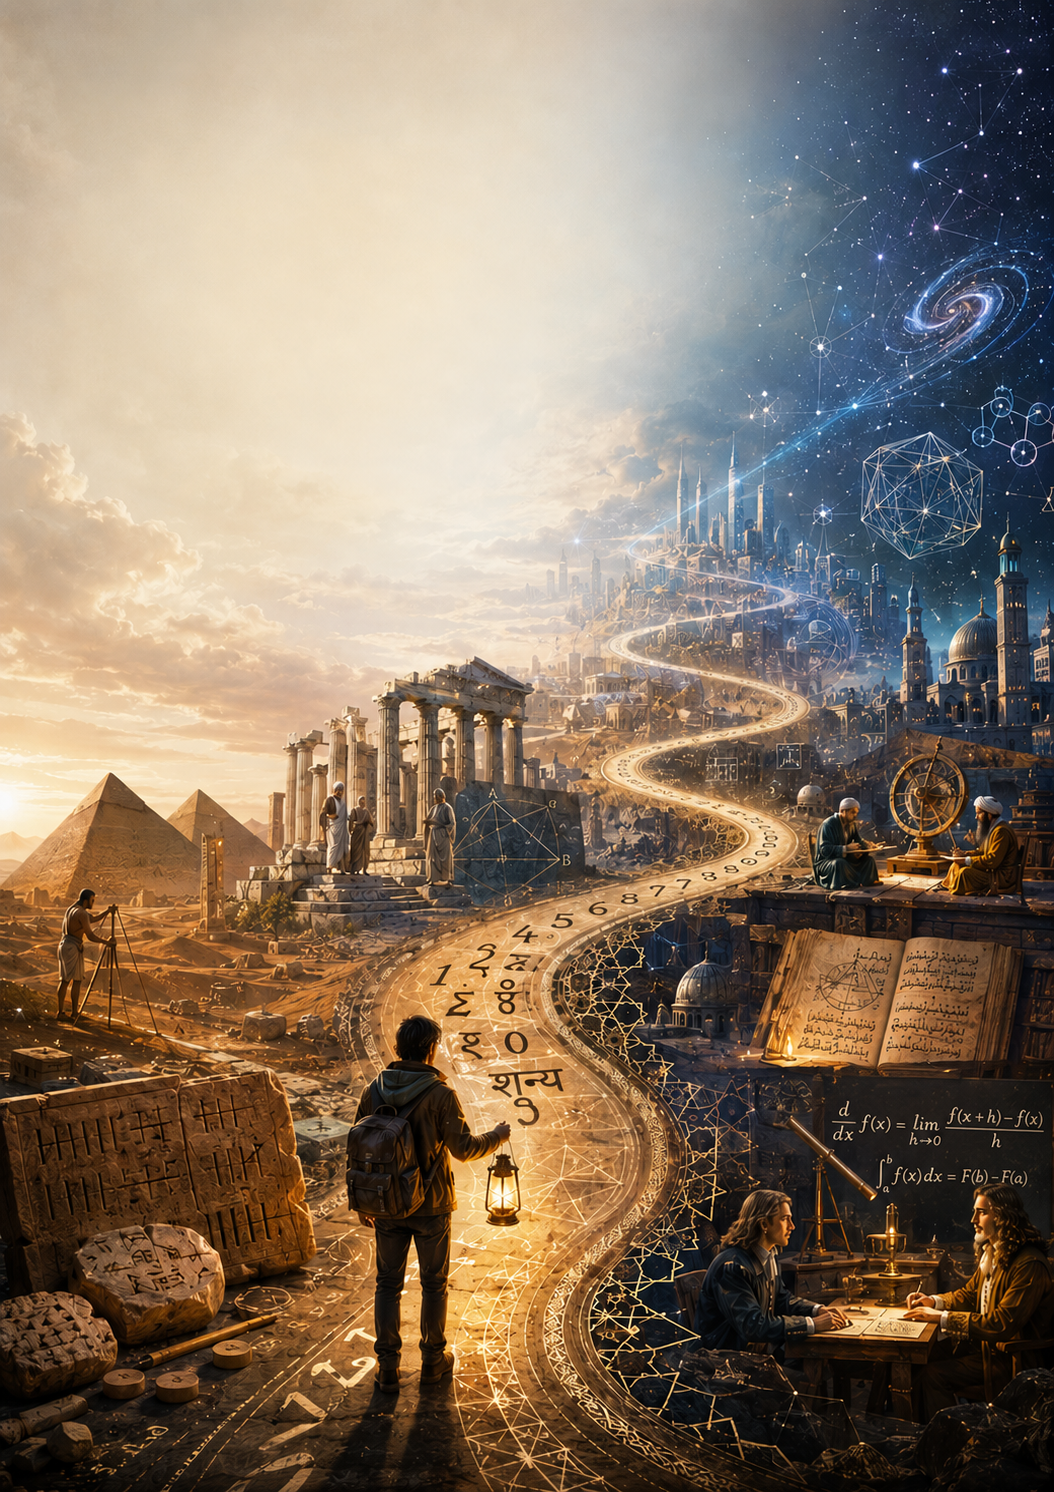
\includegraphics[width=\paperwidth, height=\paperheight]{./Images/cover.png}
\end{titlepage}

\frontmatter
\maketitle
\pagestyle{empty}
\tableofcontents
\listoffigures

\chapter{پیشگفتار}
\begin{quote}
	{\lotus
		ما باید بدانیم. ما خواهیم دانست.%
		\LTRfootnote{ Wir müssen wissen. Wir werden wissen.}
		 - دیوید هیلبرت
	}
\end{quote}
تا حالا فکر کرده‌اید که دانش ریاضی امروزی ما از کجا آمده است؟ ما چطور به اینجا رسیده‌ایم؟ من زیاد فکر کرده‌ام و بارها از خودم پرسیده‌ام. در نهایت به خودم گفتم با نشستن و فکر کردن که به جواب نمی‌رسم. باید بروم سراغ تاریخ ریاضی و البته کمی عمیق‌تر؛ شاید یک سفر ریاضی. اگر شما هم به چنین سفری علاقه‌مند هستید، می‌توانید هم‌سفر من باشید و در لذت کشف دوباره‌ی ریاضی شریک شوید.

درباره‌ی این موضوع که ما چه نیازی به ریاضی داریم حرف زیادی نمی‌زنم. کافی است به اطرافتان نگاه کنید. چیزی جز ریاضی می‌بینید؟ ریاضی زبان طبیعت است. من می‌خواهم بدانم جهان چگونه کار می‌کند و طبیعتاً باید ابتدا زبان آن را بفهمم. به علاوه، از ریاضی لذت می‌برم. همین اندازه برایم کافی است. شما بروید دلایل خودتان را پیدا کنید. من که انگیزه‌ی خودم را از این سفر پیدا کردم.

اگر انگیزه‌ی خودتان را یافتید و تصمیم گرفتید با من هم‌سفر شوید، لازم است پیش از آغاز سفر کمی درباره‌ی آن توضیح دهم. در حقیقت فقط یک چیز را می‌دانم، این که من نیز چیز زیادی نمی‌دانم. قرار است به نقطه‌ی آغاز برویم و از آنجا سفرمان را شروع کنیم. صادقانه بگویم که نمی‌دانم این سفر سرانجام دارد یا نه؛ اما می‌ارزد. اینجا شاید شک کنید که اصلاً چرا مثل دیگران نمی‌نشینیم تا فقط مطالب منسجم و مرتب کتاب‌های درسی را بخوانیم؟ این مشابه پرسش «چرا تاریخ می‌خوانیم؟» است. اگر هنوز درگیر این سؤال هستید، هنوز برای سفر آماده نیستید. در حوزه‌ی خاص ریاضی، مطالعه‌ی تاریخ فقط حفظ کردن زندگی‌نامه‌ها و دانستن زمان وقوع رخدادها نیست، بلکه فهمیدن سیر تحول و تطور آن است.

خب شاید اینجا لازم باشد هم‌سفر دیگری هم انتخاب کنیم. ابزارها بخش مهمی از زندگی ما شده‌اند و مدل‌های هوش مصنوعی نیز نوعی ابزارند. فعلاً برای اینکه با هم آشنا شوید، از ChatGPT خواستم برایتان با موضوع «چرا تاریخ ریاضی؟» سخنرانی کند و کمی هم درباره‌ی سفرمان حرف بزند. راستی تصویر جلد هم ساخته‌ی این مدل است. در ادامه نیز از این مدل و مدل هوش مصنوعی DeepSeek کمک خواهیم گرفت.

{\estedad \small
اگر بخواهیم ریاضی را تنها از روی کتاب‌های درسی بشناسیم، با جهانی روبه‌رو می‌شویم که در آن همه چیز از پیش آماده است. عددها وجود دارند، فرمول‌ها نوشته شده‌اند، قضیه‌ها اثبات شده‌اند و کافی است آن‌ها را یاد بگیریم. اما آیا ریاضیات همیشه چنین بوده است؟ روزی هیچ‌کس نمی‌دانست عدد چیست. روزی کسی نمی‌دانست چگونه زمین را اندازه بگیرد. روزی مفهوم صفر وجود نداشت، معادلات حل نمی‌شدند و حتی زبان مشترکی برای نوشتن اندیشه‌های ریاضی در دسترس نبود. ریاضیات از آسمان نازل نشده است. این دانش در طول هزاران سال و به دست انسان‌هایی شکل گرفته که با پرسش‌ها و مشکلات واقعی روبه‌رو بوده‌اند. کشاورزی که می‌خواست زمین خود را اندازه بگیرد، بازرگانی که می‌خواست حساب کالاهایش را نگه دارد، ستاره‌شناسی که حرکت سیارات را دنبال می‌کرد و اندیشمندی که در پی فهم نظم جهان بود، همگی در ساختن این بنای بزرگ سهم داشته‌اند.

پس چرا تاریخ ریاضی را می‌خوانیم؟ نه برای حفظ کردن تاریخ‌ها و نام‌ها. نه برای اینکه دوباره همه‌ی دستاوردهای گذشته را از نو اختراع کنیم. بلکه برای اینکه بفهمیم ایده‌های ریاضی چگونه متولد شده‌اند. وقتی بدانیم یک مفهوم از چه پرسشی زاده شده است، آن را بهتر درک می‌کنیم. وقتی ببینیم انسان‌ها چگونه گام‌به‌گام به یک راه‌حل رسیده‌اند، ریاضیات از مجموعه‌ای از فرمول‌های خشک به داستانی از کنجکاوی و کشف تبدیل می‌شود.

ما نمی‌خواهیم صرفاً درباره‌ی ریاضیات بخوانیم، بلکه می‌خواهیم تا حد امکان آن را همراه با سازندگانش تجربه کنیم. می‌خواهیم به روزگاری سفر کنیم که هنوز بسیاری از پاسخ‌های امروزی وجود نداشتند و جهان پر از پرسش‌های حل‌نشده بود.%
\RTLfootnote{
البته خیلی از پرسش‌ها نیز وجود نداشتند. یادتان باشد گاهی پرسش‌ها مهم‌تر از پاسخ‌ها هستند. در طول سفر، حواستان به پرسش‌ها هم باشد. به این که چرا فلان سؤال پرسیده شد و چطور سؤال درست، ما را به پاسخ درست رساند و چطور پاسخ، ما را به پرسش دیگری هدایت کرد.
}
بنابراین، این سفر برای فهم عمیق‌تر حال است. هرچه بیشتر مسیر شکل‌گیری ریاضیات را بشناسیم، بهتر می‌توانیم زیبایی، قدرت و خلاقیت نهفته در آن را درک کنیم. پس کوله‌بار کنجکاوی را بردار، هم‌سفر! راهی طولانی پیش رو داریم؛ سفری از نخستین نشانه‌های شمارش تا بلندترین قله‌های اندیشه‌ی ریاضی بشر.
}

با هم‌سفر غیرانسانی‌مان آشنا شدید و سخنانش را خواندید. من نیز چند جمله اضافه می‌کنم. یکی از مهم‌ترین اهداف آموزش ریاضی، پرورش تفکر ریاضی است. اگر این هدف را دنبال کنیم، دیگر به دنبال آموزش حافظه‌محور نخواهیم رفت. شیوه‌ی آموزش سنتی عمدتاً بر پایه‌ی حافظه است که تربیت افرادی بدون تفکر را به دنبال دارد. ما باید فکر کنیم. باید شک کنیم و باید بپرسیم. «آموزش ریاضی برای پرورش تفکر ریاضی و خلاقیت، نیازمند عبور از حافظه‌محوری به سوی تفکرورزی، کشف و تجربه است. تا زمانی که امتحان‌ها بر حفظیات استوار باشند، نمی‌توان انتظار داشت افراد تفکر ریاضی را تجربه کنند.»%
\RTLfootnote{ مجید میرزاوزیری (مصاحبه با ایسنا)}
نکته‌ی دیگر این‌که لازم است یاد بگیریم که چگونه یاد بگیریم. در این صورت است که مسیر یادگیری را سریع‌تر و با بازدهی بیشتر طی می‌کنیم. پرداختن به این موضوع هدف ما در این سفر نیست. در این راستا، شاید مطالعه‌ی کتاب «یادگیریِ یادگیری»%
  \LTRfootnote{ Learning How To Learn}
یا دیدن دوره‌ی آن در وبسایت Coursera مفید باشد.

انتظار ندارید که بدون راهنما وارد این سفر شویم؟ اگر حافظ شیرازی درباره‌ی عشق سروده است که «به کوی عشق منه بی‌دلیلِ راه قدم / که من به خویش نمودم صد اهتمام و نشد»، ما هم این را برای ریاضی می‌گوییم! من ویرایش سوم کتاب
\textbf{تاریخ ریاضی - یک مقدمه}%
\LTRfootnote{ A History of Mathematics – An Introduction}
نوشته‌ی
\textbf{ویکتور کاتز}%
\LTRfootnote{ Victor Joseph Katz}
را به عنوان راهنمای اصلی برای سفرمان انتخاب کرده‌ام. ویکتور کاتز استاد بازنشسته‌ی دانشگاه منطقه‌ی کلمبیا%
\LTRfootnote{ University of the District of Columbia (UDC)}
است و او در حوزه‌ی تاریخ ریاضی شناخته‌شده است. در این سفر بر مبنای کتاب کاتز پیش می‌رویم و به نوعی رهبری سفرمان را به او می‌سپاریم. شاید بد نباشد که فهرست کتاب او را بخوانیم تا دید کلی از سفر خود به دست آوریم.
\\
\\
\textbf{بخش ۱: ریاضیات باستانی}
\\ فصل ۱: مصر و میان‌رودان
\\ فصل ۲: آغاز ریاضیات در یونان
\\ فصل ۳: اقلیدس
\\ فصل ۴: ارشمیدس و آپولونیوس
\\ فصل ۵: روش‌های ریاضی در عصر هلنیستی
\\ فصل ۶: فصل‌های پایانی ریاضیات یونانی
\\
\\
\textbf{بخش ۲: ریاضیات قرون وسطی}
\\ فصل ۷: چین باستان و قرون وسطی
\\ فصل ۸: هند باستان و قرون وسطی
\\ فصل ۹: ریاضیات اسلام
\\ فصل ۱۰: ریاضیات در اروپای قرون وسطی
\\ فصل ۱۱: ریاضیات در سراسر جهان
\\
\\
\textbf{بخش ۳: ریاضیات دوره‌ی آغازین مدرن}%
\LTRfootnote{ Early Modern Mathematics}
\\ فصل ۱۲: جبر در رنسانس
\\ فصل ۱۳: روش‌های ریاضی در رنسانس
\\ فصل ۱۴: جبر، هندسه، و احتمال در قرن هفدهم
\\ فصل ۱۵: آغاز حسابان (حساب دیفرانسیل و انتگرال)
\\ فصل ۱۶: نیوتون و لایبنیتس
\\
\\
\textbf{بخش ۴: ریاضیات مدرن}
\\ فصل ۱۷: آنالیز در قرن هجدهم
\\ فصل ۱۸: احتمال و آمار در قرن هجدهم
\\ فصل ۱۹: جبر و نظریه‌ی اعداد در قرن هجدهم
\\ فصل ۲۰: هندسه در قرن هجدهم
\\ فصل ۲۱: جبر و نظریه‌ی اعداد در قرن نوزدهم
\\ فصل ۲۲: آنالیز در قرن نوزدهم
\\ فصل ۲۳: احتمال و آمار در قرن نوزدهم
\\ فصل ۲۴: هندسه در قرن نوزدهم
\\ فصل ۲۵: جنبه‌هایی از قرن بیستم و فراتر از آن
\\
\\
به نظرم دیگر آماده‌ی سفر شده‌ایم. آماده‌اید؟



\begin{flushleft}
	{\lotus
	مژگان به کارخانه‌ی حیرت گشوده‌ایم \\
	در دستِ ما کلیدِ درِ باز داده‌اند \\
	«بیدل دهلوی»
}
\end{flushleft}
\pagestyle{fancy}

\mainmatter
\chapter{مصر باستان}

به نقطه‌ی آغاز سفر خوش آمدید. بیایید سری به موزه‌ی بریتانیا بزنیم تا یک متن کهن را ببینیم، پاپیروس ریاضی رایند%
\LTRfootnote{ Rhind Mathematical Papyrus}.
قدمت این پاپیروس به حدود ۱۵۵۰ سال پیش از میلاد می‌رسد و متعلق به مصر باستان است. نترسید، نمی‌خواهیم الآن آن را بخوانیم! فقط جالب است بدانید با چه عبارتی شروع می‌شود. «محاسبه‌ی دقیق؛ راهیابی به دانش همه‌ی چیزهای موجود و شناخت همه‌ی رازها و اسرار نهفته.»
\begin{figure}[h]
	\centering
	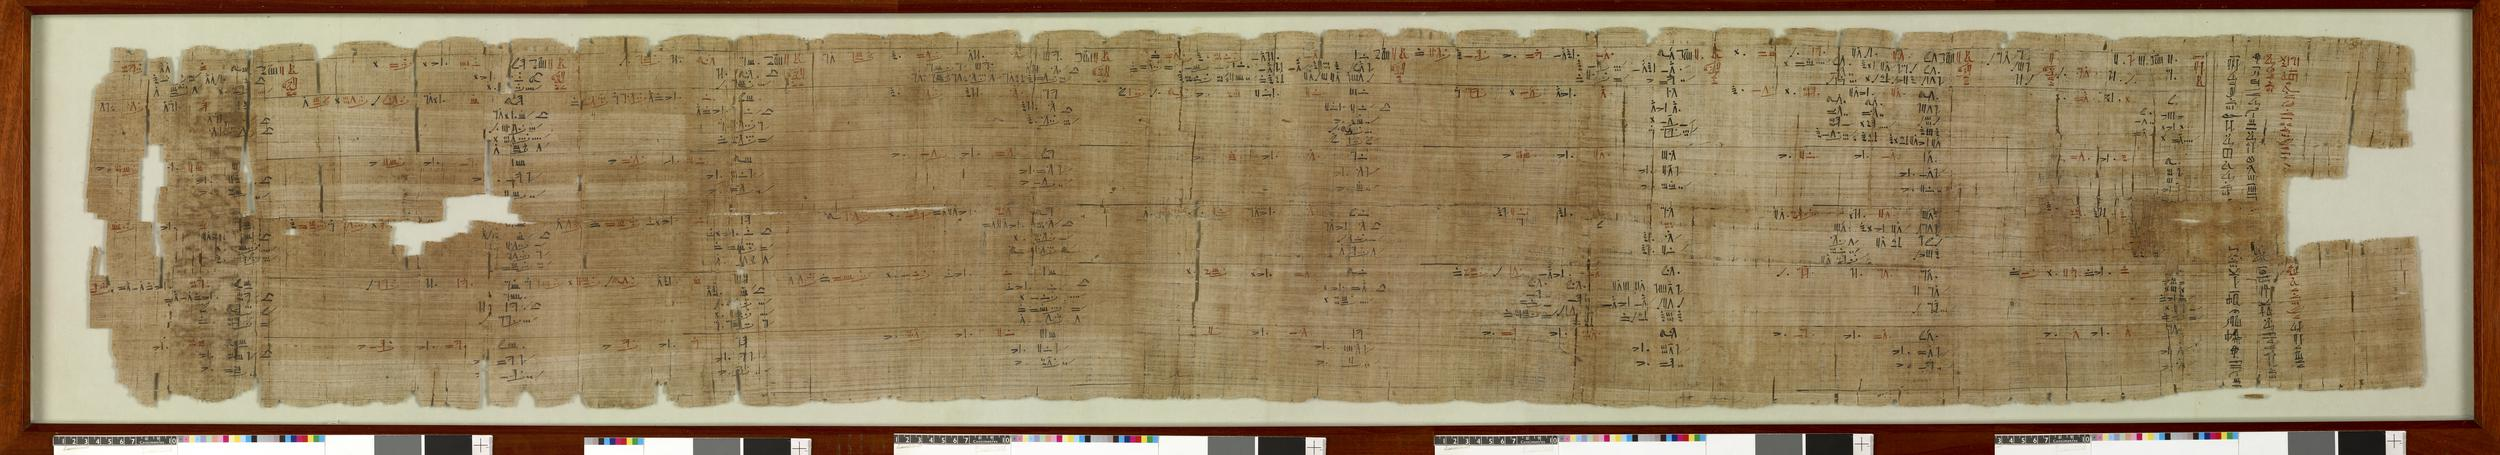
\includegraphics[width=\textwidth]{./Images/366139001.jpg}
	\caption{پاپیروس ریاضی رایند}
	\label{fig1.1}
\end{figure}

%%%%%%%%%%%%%%%%%%%%%%%%%%%%%%%%%%%%%%%%%%%%%%
\section{سیستم‌های عددی و محاسبات}

کمی عقب‌تر برویم، به ۳۱۰۰ سال پیش از میلاد. نوشتار در مصر تقریباً در همین دوران آغاز شد و بیشتر نوشته‌های اولیه به حسابداری و ثبت انواع کالاها مربوط می‌شد. از همان ابتدای پیدایش خط در مصر، دو سبک نوشتاری وجود داشت: خط هیروگلیف برای نوشتن معمولاً روی دیوارها و ستون‌ها و تندیس‌ها و خط هیراتیک برای نوشتن روزمره معمولاً روی پاپیروس. بنابراین مصری‌ها دو سیستم عددنویسی مختلف نیز داشتند، سیستم هیروگلیف و سیستم هیراتیک. در سیستم هیروگلیف هر توان ۱۰ با یک نماد نشان داده می‌شود.
\begin{figure}[h]
	\centering
	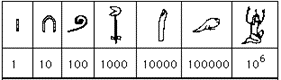
\includegraphics[width=0.5\textwidth]{./Images/Hieroglyph.png}
	\caption{سیستم عددنویسی هیروگلیف}
	\label{fig1.2}
\end{figure}

اما اعداد در سیستم هیروگلیف چطور نوشته می‌شوند؟ نظرتان چیست که خودتان کشف کنید؟ من سه تا تصویر واقعی نشان شما می‌دهم و شما به کمک شکل \ref{fig1.2} تلاش کنید که بفهمید هر کدام چه عددی را نشان می‌دهند.
\begin{figure}[h]
	\centering
	\begin{subfigure}{0.3\textwidth}
		\centering
		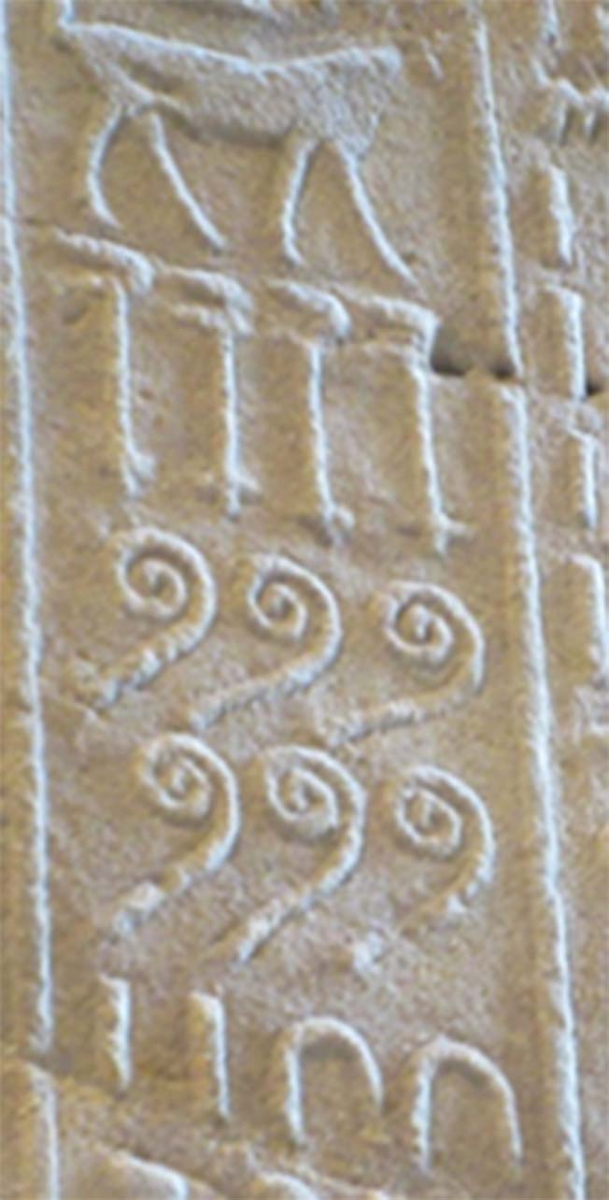
\includegraphics[height=2in, keepaspectratio=true]{./Images/Huffman_Egypt-Fig5-Louvre.jpg}
		\caption{لوور}
		\label{fig1.3.1}
	\end{subfigure}
	\hspace{0.03\textwidth}
	\begin{subfigure}{0.3\textwidth}
		\centering
		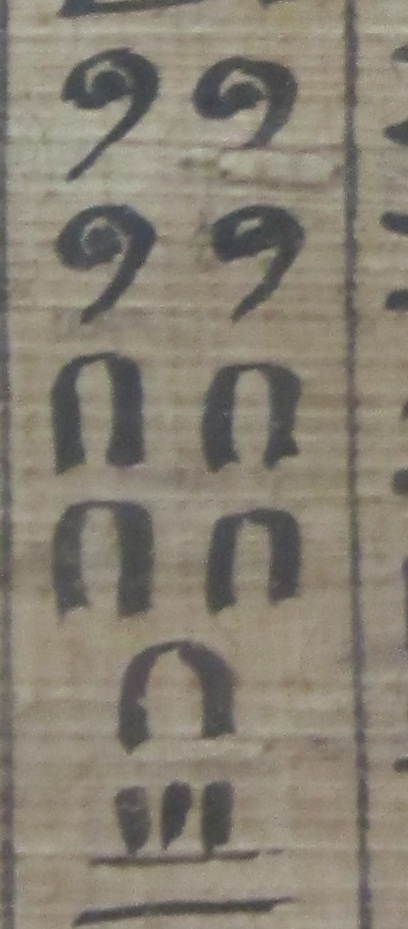
\includegraphics[height=2in, keepaspectratio=true]{./Images/Huffman_Egypt-Fig6b-Turin.jpg}
		\caption{تورین}
		\label{fig1.3.2}
	\end{subfigure}
	\hspace{0.03\textwidth}
	\begin{subfigure}{0.3\textwidth}
		\centering
		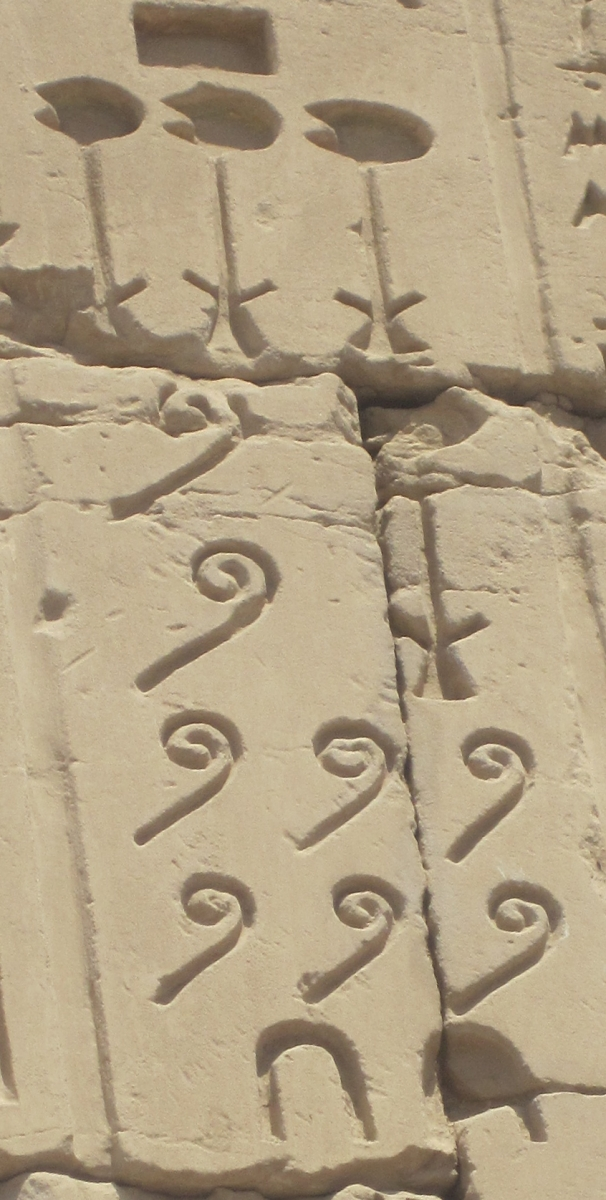
\includegraphics[height=2in, keepaspectratio=true]{./Images/Huffman_Egypt-Fig7a-Karnak.jpg}
		\caption{کارنک}
		\label{fig1.3.3}
	\end{subfigure}
	
	\caption{نمونه‌ی هیروگلیف‌های عددی}
	\label{fig1.3}
\end{figure}

شکل \ref{fig1.3} شامل سه متن هیروگلیف مختلف است. تصویر سمت راست، مربوط به سال‌نامه‌ی توتمس سوم در معبد کارنَک در شهر الأقصر مصر است که اکنون در موزه‌ی لوور شهر پاریس نگهداری می‌شود و عدد ۴۶۲۲ را نمایش می‌دهد. تصویر وسط، مربوط به یک پاپیروس است که در شهر تورین ایتالیا نگهداری می‌شود و عدد ۴۵۳ را نمایش می‌دهد. تصویر سمت چپ، دیواری در معبد کارنک است که عدد ۴۸۲۰ را نمایش می‌دهد. آیا به راز آن‌ها پی بردید؟ کافی است تعداد هر نماد را بشمارید تا رقم مربوط به هر جایگاه را بیابید. به ترتیب قرار گرفتن نمادها نیز دقت کنید. نماد توان بزرگتر، بالاتر یا در سمت راست قرار می‌گیرد. همچنین، نوشته را از بالا به پایین یا از راست به چپ می‌نویسند. حالا می‌توانید دو عدد ۷۸۳ و ۲۷۵ را در سیستم هیروگلیف بنویسید؟

سیستم هیراتیک روش متفاوتی برای عددنویسی دارد. در این سیستم، هر رقم ۱ تا ۹ نماد خاصی دارد. همچنین، هر عدد مضرب ۱۰ از ۱۰ تا ۹۰، هر عدد مضرب ۱۰۰ از ۱۰۰ تا ۹۰۰ و ... هر کدام دارای نماد خاصی هستند. برای مثال، برای نوشتن عدد ۳۷ کافی است ۳۰ و ۷ را کنار هم بنویسیم.
\begin{figure}[h]
	\centering
	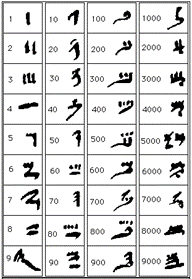
\includegraphics[width=0.4\textwidth]{./Images/Hieratic.png}
	\caption{سیستم عددنویسی هیراتیک}
	\label{fig1.4}
\end{figure}

خب تا اینجای سفر چطور بود؟ امیدوارم اوایلش خسته‌کننده نباشد، چون با مفاهیم ابتدایی سروکار داریم. به دو عمل جمع و تفریق نمی‌پردازیم چون کار آسانی است. خودتان امتحان کنید. دو عدد ۷۸۳ و ۲۷۵ را که نوشته بودید، یک بار با هم جمع کنید و یک بار از هم کم کنید. حال به سراغ ضرب و تقسیم می‌رویم که دیگر به راحتی جمع و تفریق نیست.

الگوریتم مصری برای ضرب بر پایه‌ی فرایند دو برابر کردن متوالی است. بگذارید با یک مثال توضیح دهم. فرض کنید می‌خواهیم ۱۲ را در ۱۳ ضرب کنیم. یک جدول دو ستونی تشکیل می‌دهیم و ۱ و ۱۲ را در ردیف اول می‌نویسیم. حال هر کدام را در ۲ ضرب می‌کنیم و در ردیف بعدی می‌نویسیم. به محض این‌که عدد سمت چپ مساوی ۱۳ یا بزرگتر شد، فرایند را متوقف می‌کنیم و آن ردیف را حذف می‌کنیم. حال با عددهای ستون چپ، عدد ۱۳ را می‌سازیم، یعنی با جمع ۱، ۴ و ۸. سپس عدد متناظر هر کدام در ستون راست را با هم جمع می‌کنیم، یعنی ۱۲، ۴۸ و ۹۶ که جمعشان برابر با ۱۵۶ می‌شود. به حاصل ۱۲ ضرب در ۱۳ رسیدیم.



%%%%%%%%%%%%%%%%%%%%%%%%%%%%%%%%%%%%%%%%%%%%%%
\section{معادلات خطی و استدلال تناسبی}

بر اساس پاپیروس‌های رایند و مسکو می‌دانیم که مصری‌ها با مسائلی مواجه بودند که ما امروزه آن‌ها را معادلات خطی، تناسب‌ها، و هندسه می‌نامیم.
\include{./TeX_files/chapter02}

\cleardoublepage
\addcontentsline{toc}{chapter}{مراجع}

\renewcommand{\bibname}{مراجع}
\begin{thebibliography}{99}
	\begin{LTRbibitems}
		\resetlatinfont
		\bibitem{EngRef1}
		Katz, V. J. (2009). A History of Mathematics - An Introduction (3rd ed.). Boston: Pearson Education, Inc.
		\bibitem{EngRef2}
		https://old.maa.org/press/periodicals/convergence/an-ancient-egyptian-mathematical-photo-album-counting-numbers
		\bibitem{EngRef3}
		ref
	\end{LTRbibitems}
	\bibitem{PerRef1}
	منبع فارسی شمارۀ یک.
\end{thebibliography}

\cleardoublepage
\chapter*{منابع تصاویر}
\addcontentsline{toc}{chapter}{منابع تصاویر}
شکل \ref{fig1.1}
\dotfill
\lr{©The Trustees of the British Museum. Shared under a CC BY-NC-SA 4.0 license.}
\\
%%%%%%%%%%%%%%%%%%%%%%%%%%%%%%%%%%
شکل \ref{fig1.2}
\dotfill
\href{https://mathshistory.st-andrews.ac.uk/HistTopics/Egyptian_numerals/}{mathshistory.st-andrews}
\\
%%%%%%%%%%%%%%%%%%%%%%%%%%%%%%%%%%
شکل \ref{fig1.3}
\dotfill
\lr{Photos by \href{https://old.maa.org/press/periodicals/convergence/an-ancient-egyptian-mathematical-photo-album-counting-numbers}{Cynthia J. Huffman}. Shared under a CC BY 4.0 license.}
\\
%%%%%%%%%%%%%%%%%%%%%%%%%%%%%%%%%%
شکل \ref{fig1.4}
\dotfill
\href{https://mathshistory.st-andrews.ac.uk/HistTopics/Egyptian_numerals/}{mathshistory.st-andrews}
\\
%%%%%%%%%%%%%%%%%%%%%%%%%%%%%%%%%%
\chapter*{واژه‌نامه‌ی فارسی - انگلیسی}
\addcontentsline{toc}{chapter}{واژه‌نامه‌ی فارسی - انگلیسی}
%%%%%%%%%%%%%%%%%%%%%%%%%%%%%%%
پاپیروس ریاضی رایند
\dotfill 
\lr{Rhind Mathematical Papyrus}
\\
%%%%%%%%%%%%%%%%%%%%%%%%%%%%%%%
ریاضیات دوره‌ی آغازین مدرن
\dotfill 
\lr{Early Modern Mathematics}
\\
%%%%%%%%%%%%%%%%%%%%%%%%%%%%%%%
کسر با صورت ۱
\dotfill
\lr{Unit Fraction}
\\
%%%%%%%%%%%%%%%%%%%%%%%%%%%%%%%
عدد مخلوط
\dotfill
\lr{Mixed Number}
\\
%%%%%%%%%%%%%%%%%%%%%%%%%%%%%%%
عدد کامل
\dotfill
\lr{Whole Number}
\\
%%%%%%%%%%%%%%%%%%%%%%%%%%%%%%%
معادله‌ی خطی
\dotfill
\lr{Linear Equation}
\\
%%%%%%%%%%%%%%%%%%%%%%%%%%%%%%%
تناسب
\dotfill
\lr{Proportion}
\\
%%%%%%%%%%%%%%%%%%%%%%%%%%%%%%%
هندسه
\dotfill
\lr{Geometry}
\\
%%%%%%%%%%%%%%%%%%%%%%%%%%%%%%%
فرض غلط
\dotfill
\lr{False Position}
\\
%%%%%%%%%%%%%%%%%%%%%%%%%%%%%%%
کلمه
\dotfill
\lr{word}
\\
%%%%%%%%%%%%%%%%%%%%%%%%%%%%%%%\\
کلمه
\dotfill
\lr{word}
\\
%%%%%%%%%%%%%%%%%%%%%%%%%%%%%%%

\end{document}